% 3d-stack-two-lumped: heat-flow network, EXPANDED multi-layer view (TikZ).
% Source: config/thermal/3d-stack-two-lumped.yaml (schema v1) +
%        DomainExpert model-ruling XIV (3D representation decision,
%        thermal-g-construction Sec 2 full multi-layer form).
% Compile: pdflatex 3d-stack-two-lumped.tex   (TeX Live 2026)
%
% Each stack is expanded into per-layer die nodes (top / bottom) so the
% internal heat path is visible: inter-layer vertical = TSV/hybrid bonding
% (layer-to-layer thermal resistance), per-layer lateral face adjacency,
% and the vertical cooling chain bottom-die -> ambient (lumped R_vert =
% 2.4 K/W, 2 layers in series). Expanded view and lumped value are shown
% together.
%
% Edge styling: face_adjacency = solid blue; vertical_chain = solid amber
% arrow; TSV/hybrid bonding = dashed purple arrow; reserved: ground =
% double. All routing orthogonal (no diagonals).
\documentclass[border=10pt]{standalone}
\usepackage{sfmath}
\renewcommand{\familydefault}{\sfdefault}
\usepackage{tikz}
\usetikzlibrary{arrows.meta, shapes.geometric}
\definecolor{stkfill}{HTML}{FFF4E5}   % stack/die: light amber fill
\definecolor{stkedge}{HTML}{B45309}
\definecolor{bndfill}{HTML}{F1F3F4}   % boundary: light gray ellipse
\definecolor{bndedge}{HTML}{5F6368}
\definecolor{faedge}{HTML}{1A73E8}    % face_adjacency: solid blue
\definecolor{vcedge}{HTML}{B45309}    % vertical_chain: solid amber arrow
\definecolor{tsvedge}{HTML}{9334E6}   % TSV/hybrid bonding: dashed purple
\begin{document}
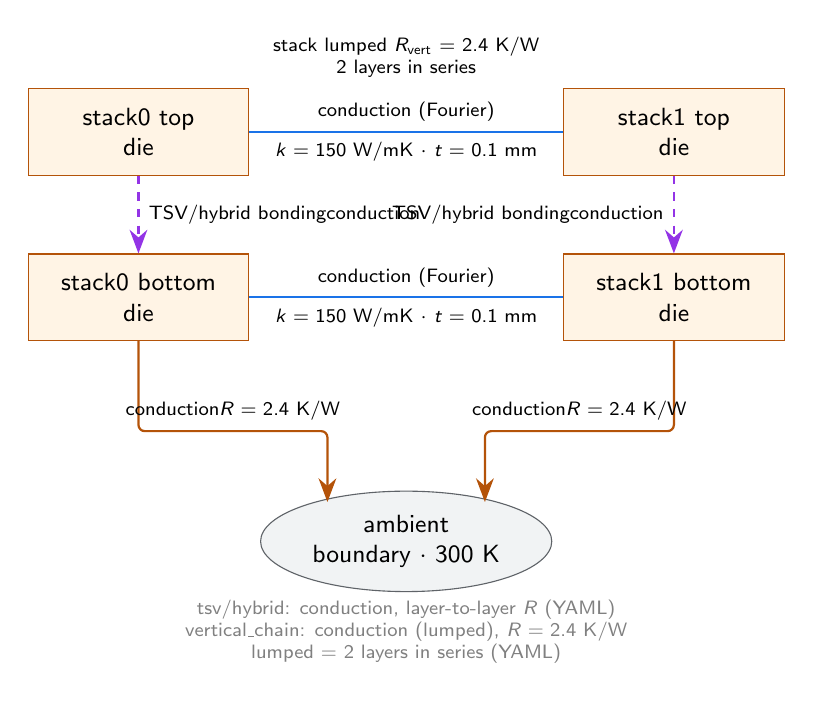
\begin{tikzpicture}[
  die/.style={rectangle, draw=stkedge, fill=stkfill, minimum width=2.8cm,
              minimum height=1.1cm, align=center, font=\small},
  bnd/.style={ellipse, draw=bndedge, fill=bndfill, minimum width=3.0cm,
              minimum height=1.1cm, align=center, font=\small},
  fa/.style={draw=faedge, thick},
  vc/.style={draw=vcedge, thick, -{Stealth[length=3mm]}, rounded corners=0.08cm},
  tsv/.style={draw=tsvedge, thick, dashed, -{Stealth[length=3mm]}},
  lab/.style={font=\scriptsize},
]
% per-layer die nodes (expanded: top / bottom)
\node[die] (t0) at (-3.4,  1.6) {stack0 top\\die};
\node[die] (t1) at ( 3.4,  1.6) {stack1 top\\die};
\node[die] (b0) at (-3.4, -0.5) {stack0 bottom\\die};
\node[die] (b1) at ( 3.4, -0.5) {stack1 bottom\\die};
\node[bnd] (ambient) at (0, -3.6) {ambient\\boundary $\cdot$ 300 K};
% per-layer lateral face adjacency (each layer independently)
\draw[fa] (t0.east) -- node[above, lab] {conduction (Fourier)}
                      node[below, lab] {$k=150$ W/mK $\cdot$ $t=0.1$ mm} (t1.west);
\draw[fa] (b0.east) -- node[above, lab] {conduction (Fourier)}
                      node[below, lab] {$k=150$ W/mK $\cdot$ $t=0.1$ mm} (b1.west);
% inter-layer vertical: TSV/hybrid bonding (layer-to-layer thermal R)
\draw[tsv] (t0.south) -- node[right, lab] {TSV/hybrid bonding\\conduction} (b0.north);
\draw[tsv] (t1.south) -- node[left, lab]  {TSV/hybrid bonding\\conduction} (b1.north);
% vertical cooling chains: bottom die -> ambient (lumped R_vert, 2 layers in series)
\draw[vc] (b0.south) -- (-3.4,-2.2) -- node[above, lab] {conduction\\$R=2.4$ K/W} (-1.0,-2.2) -- (-1.0,-3.10);
\draw[vc] (b1.south) -- ( 3.4,-2.2) -- node[above, lab] {conduction\\$R=2.4$ K/W} ( 1.0,-2.2) -- ( 1.0,-3.10);
% lumped summary: expanded view + lumped value shown together
\node[lab, align=center] at (0, 2.55) {stack lumped $R_{\mathrm{vert}}$ = 2.4 K/W\\2 layers in series};
% branch annotation: physical path type + value provenance (geometry+material)
\node[lab, align=center, text=gray] at (0, -4.75) {
  tsv/hybrid: conduction, layer-to-layer $R$ (YAML)\\
  vertical\_chain: conduction (lumped), $R=2.4$ K/W\\
  lumped = 2 layers in series (YAML)};
\end{tikzpicture}
\end{document}
